
\section{Study of Parallel Workload \Rmnum{2 }}
%\section{``Bully" become ``Bullee"}
\label{sec:workload-2}

In this section, we will verify the observations made in the previous section when Workload \Rmnum{1} is running on the dragonfly network under different placement and routing configurations. We conduct the same sets of experiments with Workload \Rmnum{2}, which consists of sAMG, MultiGrid and CrystalRouter. By replacing AMG with sAMG, we turn the ``bully" into ``bullee".

\subsection{Network Performance Analysis}
\label{sec: workload-2 network analysis}

\begin{table}[ht]
\begin{center}
\caption{Average time spent on communication by all MPI ranks when Workload II is running on dragonfly network under 6 different placement and routing configurations.} 
\label{tab:syn-wkld-commtime}
%\centering % Centers the table on the page, comment out to left-justify
\begin{tabular}{l c c c c c c }
\toprule % Top horizontal line
\toprule
&\multicolumn{6}{c}{Placement and Routing Configuration} \\ % Amalgamating several columns into one cell is done using the \multicolumn command as seen on this line
\cmidrule(l){2-7}
          & CM & CA & CPA & RM & RA & RPA \\ % Column names row
\midrule % In-table horizontal line
Time(ms)  & 3360 & 2204 & 2335 & 1791 & 2367 & 1965 \\ % Content row 1

\midrule % In-table horizontal line
\bottomrule % Bottom horizontal line
\end{tabular}
\end{center}
\end{table}


The average communication time spent by all MPI ranks when Workload \Rmnum{2} is running under different placement and routing configurations shown in Table \ref{tab:syn-wkld-commtime}. The contiguous placement coupled with minimal routing results in highest communication time. The random placement coupled with minimal routing is the most efficient. Progressive adaptive routing is better than adaptive routing when random placement is in use. And they have comparable results when coupled contiguous placement. The performance of Workload \Rmnum{2} under different configurations keep the similar pattern as it of Workload \Rmnum{1}. 


Figure \ref{fig:synwkld-network-traffic-stime} shows the aggregate traffic for terminal links, local channels and global channels, and the corresponding saturated time when Workload \Rmnum{2} is running with 6 different configurations. Contiguous placement coupled with minimal routing(CM) results in most traffic go through certain local and global channel, thus the longest saturated time for terminal link, local and global channel. When contiguous placement is coupled with (progressive) adaptive routing (CA, CPA), the local congestion could be mitigated. The random placement coupled with any routing policy(RM, RA, RPA) performs comparably. They are better than contiguous placement and minimal routing(CM), but only little improvement against contiguous and (progressive) adaptive (CA, CPA).



\begin{figure*}[t]
    \centering
    \begin{subfigure}[t]{0.32\textwidth}
        \centering
        \includegraphics[height=1.8 in]{syn-wkld/gc-traffic}
        \caption{Global Channel Traffic}
        \label{fig:synwkld-global-channel-traffic}
    \end{subfigure}\hfill
    \hspace{1em}%
    \begin{subfigure}[t]{0.32\textwidth}
        \centering
        \includegraphics[height=1.8 in]{syn-wkld/lc-traffic}
        \caption{Local Channel Traffic}
        \label{fig:synwkld-local-channel-traffic}
    \end{subfigure}\hfill
    \hspace{1em}%
    \begin{subfigure}[t]{0.32\textwidth}
        \centering
        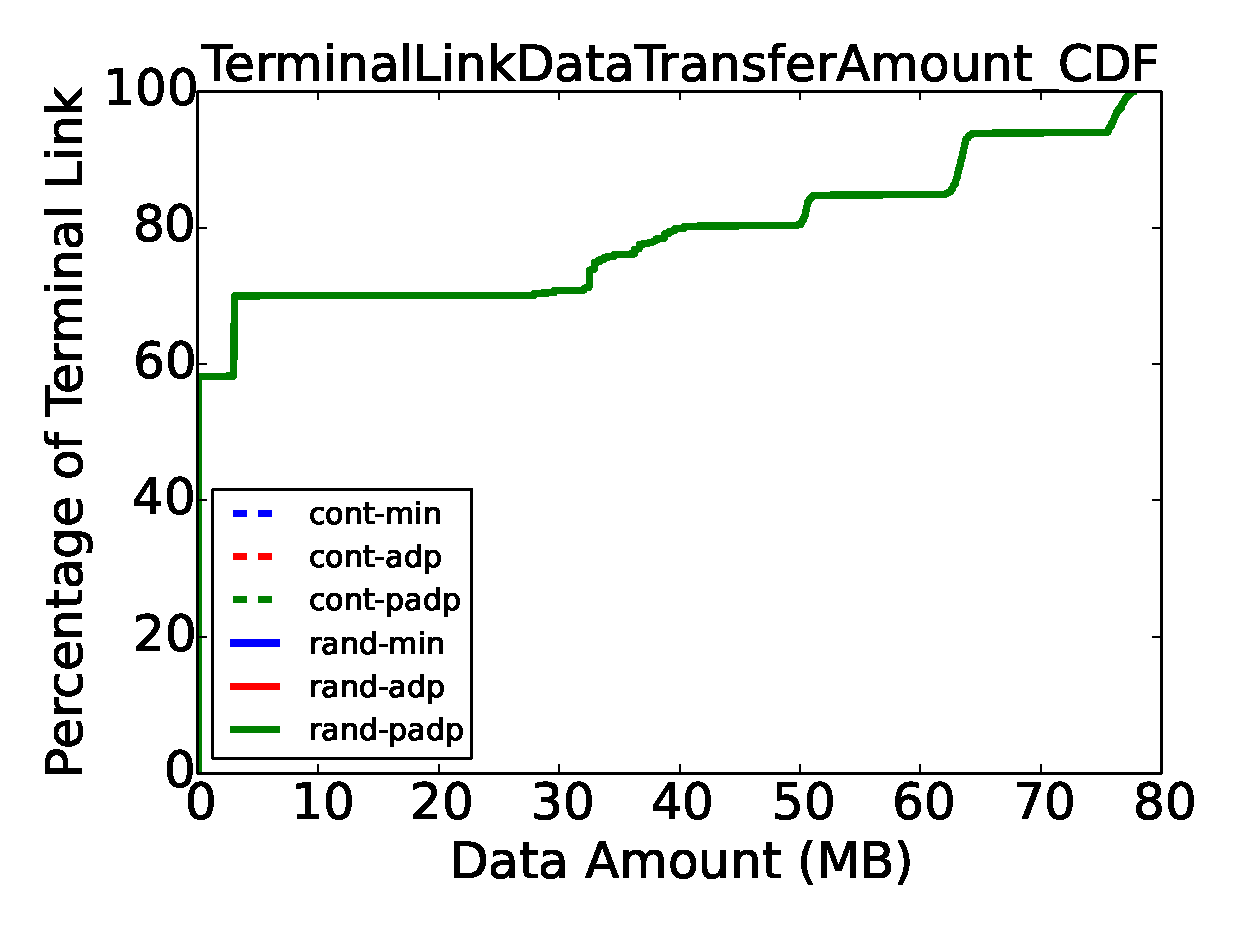
\includegraphics[height=1.8 in]{syn-wkld/tl-traffic}
        \caption{Terminal Link Traffic}
        \label{fig:synwkld-terminal-link-traffic}
    \end{subfigure}\\

    \begin{subfigure}[t]{0.32\textwidth}
        \centering
        \includegraphics[height=1.8 in]{syn-wkld/gc-btime}
        \caption{Global Channel Saturated Time}
        \label{fig:synwkld-global-channel-stime}
    \end{subfigure}\hfill
     \hspace{1em}%
    \begin{subfigure}[t]{0.32\textwidth}
        \centering
        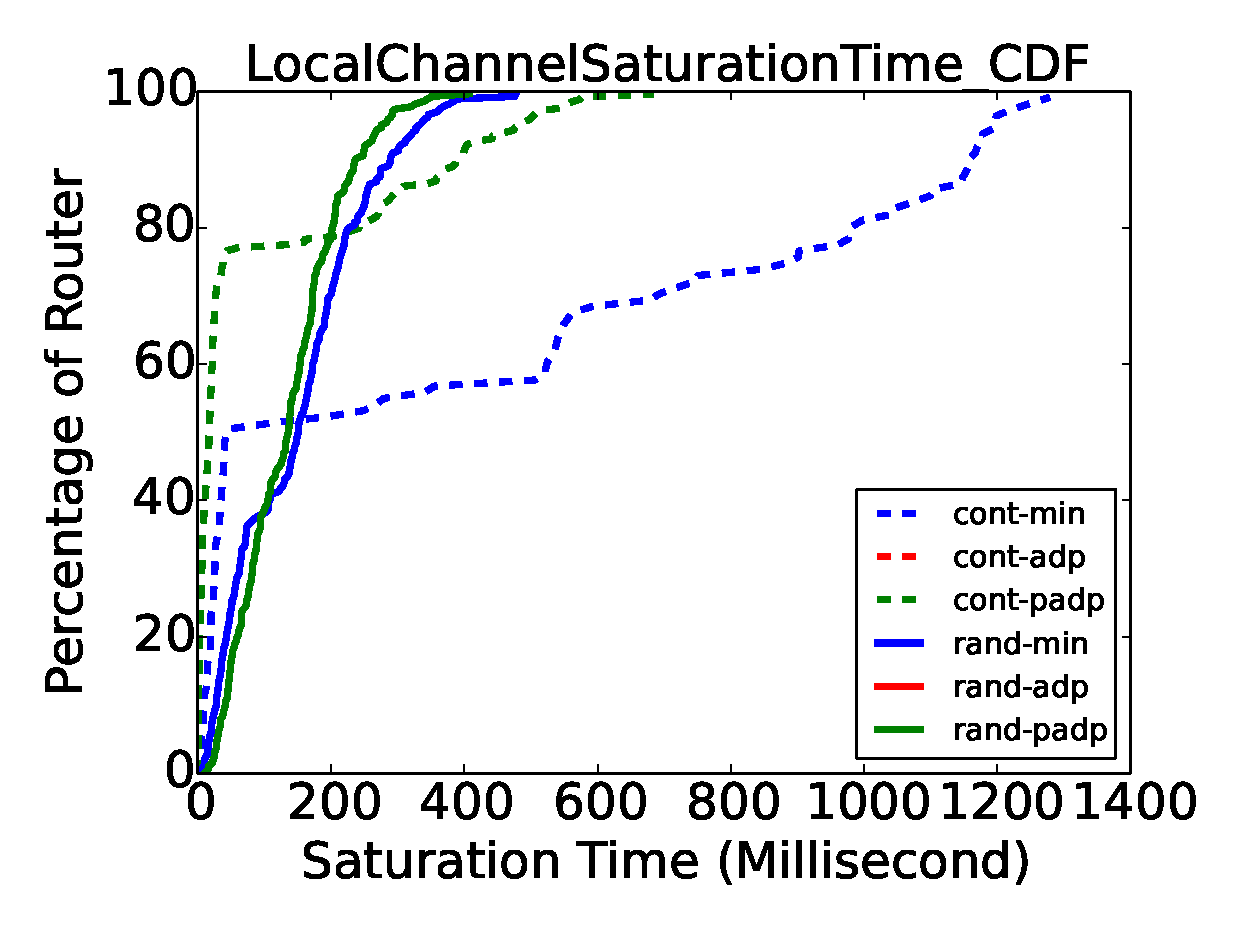
\includegraphics[height=1.8 in]{syn-wkld/lc-btime}
        \caption{Local Channel Saturated Time}
        \label{fig:synwkld-local-channel-stime}
    \end{subfigure}\hfill
    \hspace{1em}%
    \begin{subfigure}[t]{0.32\textwidth}
        \centering
        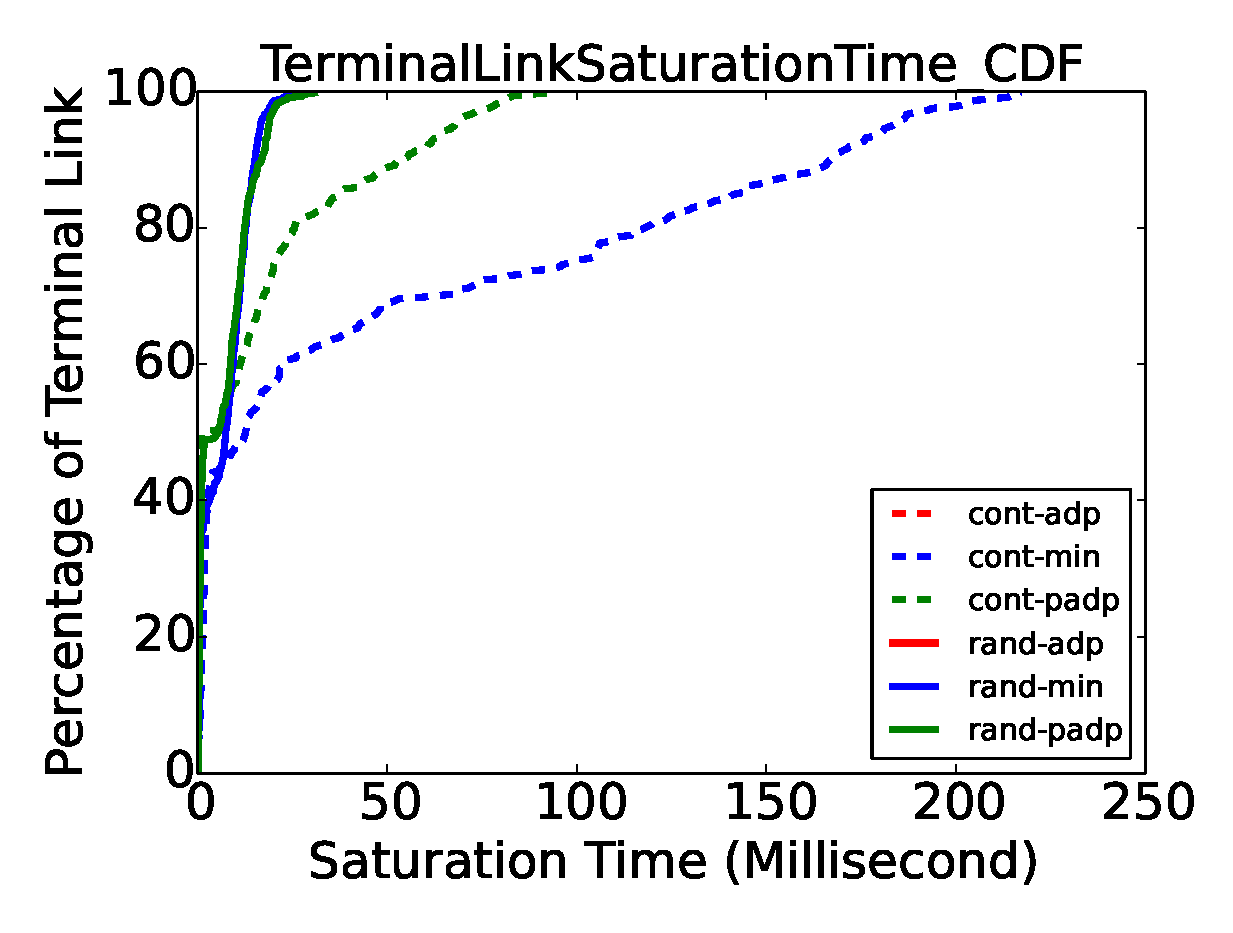
\includegraphics[height=1.8 in]{syn-wkld/tl-btime}
        \caption{Terminal Link Saturated Time}
        \label{fig:synwkld-terminal-link-stime}
    \end{subfigure}%
   \caption{Traffic and Saturated Time of different level of links in the dragonfly network when Workload \Rmnum{2} is running under 6 different placement and routing configurations.}
   \label{fig:synwkld-network-traffic-stime}
\end{figure*}

\subsection{Individual Application Analysis}
\label{sec: workload-2 app analysis}

The communication time of each application shown in Figure \ref{fig:syn-apps-commtime}. The ``bully" in Workload \Rmnum{1} becomes the ``bullyee" in Workload \Rmnum{2}. MultiGrid and CrystalRouter are the less communication-intensive applications in Workload \Rmnum{2}.  When random placement coupled with (progressive) adaptive routing is in use, MultiGrid and CrystalRouter suffer prolonged communication time, shown in Figure \ref{fig:syn-mg-commtime}, \ref{fig:syn-cr-commtime}. Whereas, sAMG benefits from random placement and (progressive) adaptive routing, shown in Figure \ref{fig:syn-samg-commtime}. Contiguous placement coupled with minimal routing prevents applications from sharing network resource, guaranteeing the performance of less communication intensive applications like MultiGrid and CrystalRouter and causing severe performance degradation to sAMG.

\begin{figure*}[t!]
    \centering
    \begin{subfigure}[t]{0.32\textwidth}
        \centering
        \includegraphics[height=1.5 in]{syn-wkld/amg10/commtime}
        \caption{sAMG}
        \label{fig:syn-samg-commtime}
    \end{subfigure}%
    \hspace{1em}%
    \begin{subfigure}[t]{0.32\textwidth}
        \centering
        \includegraphics[height=1.5 in]{syn-wkld/mg/commtime}
        \caption{MultiGrid}
        \label{fig:syn-mg-commtime}
    \end{subfigure}%
    \begin{subfigure}[t]{0.32\textwidth}
        \centering
        \includegraphics[height=1.5 in]{syn-wkld/cr/commtime}
        \caption{CrystalRouter}
        \label{fig:syn-cr-commtime}
    \end{subfigure}%
   \caption{The communication time of all ranks in each application. Three applications running concurrently on dragonfly network with different placement and routing configurations. The ``bully", sAMG, benefits from random placement and adaptive routing, while the ``bullee", MultiGrid and CrystalRouter, suffer performance degradation.}
   \label{fig:syn-apps-commtime}
\end{figure*}

% explain the network status of sAMG, MG and CR
We look into the network level to scrutinize the traffic through the routers serving each application. Figure \ref{fig:syn-samg-lc-traffic}, \ref{fig:syn-samg-gc-traffic} shows the traffic go through the local and global channels of the routers serving sAMG. The traffic skyrockets in both local and global channels when contiguous placement coupled with minimal routing (CM) is in use. The congestion will be alleviated in both local and global channels when contiguous placement coupled with (progressive) adaptive routing (CA, CPA) are in use. Random placement can further reduce the traffic burden on local and global channels by uniformly distributing sAMG traffic over the network. 

The traffic go through the local and global channels of the routers serving MultiGrid and CrystalRouter are shown in Figure \ref{fig:syn-mg-lc-traffic}, \ref{fig:syn-mg-gc-traffic} and Figure \ref{fig:syn-cr-lc-traffic}, \ref{fig:syn-cr-gc-traffic}. There are more traffic going through when random placement is in use, compared with contiguous placement. The extra traffic coming from the ``bully" sAMG cause performance degradation to MultiGrid and CrystalRouter. 


\begin{figure*}[t]
    \centering
    \begin{subfigure}[t]{0.32\textwidth}
        \centering
        \includegraphics[height=1.5 in]{syn-wkld/amg10/lc-traffic}
        \caption{sAMG Local Channel Traffic}
        \label{fig:syn-samg-lc-traffic}
    \end{subfigure}\hfill
    \hspace{1em}%
    \begin{subfigure}[t]{0.32\textwidth}
        \centering
        \includegraphics[height=1.5 in]{syn-wkld/mg/lc-traffic}
        \caption{MG Local Channel Traffic}
        \label{fig:syn-mg-lc-traffic}
    \end{subfigure}\hfill
    \begin{subfigure}[t]{0.32\textwidth}
        \centering
        \includegraphics[height=1.5 in]{syn-wkld/cr/lc-traffic}
        \caption{CR Local Channel Traffic}
        \label{fig:syn-cr-lc-traffic}
    \end{subfigure}\\
    \centering
    \begin{subfigure}[t]{0.32\textwidth}
        \centering
        \includegraphics[height=1.5 in]{syn-wkld/amg10/gc-traffic}
        \caption{sAMG Global Channel Traffic}
        \label{fig:syn-samg-gc-traffic}
    \end{subfigure}\hfill
    \hspace{1em}%
    \begin{subfigure}[t]{0.32\textwidth}
        \centering
        \includegraphics[height=1.5 in]{syn-wkld/mg/gc-traffic}
        \caption{MG Global Channel Traffic}
        \label{fig:syn-mg-gc-traffic}
    \end{subfigure}\hfill
    \begin{subfigure}[t]{0.32\textwidth}
        \centering
        \includegraphics[height=1.5 in]{syn-wkld/cr/gc-traffic}
        \caption{CR Global Channel Traffic}
        \label{fig:syn-cr-gc-traffic}
    \end{subfigure}%
   \caption{The aggregate traffic go through the local and global channels of routers serving specific application. ``CA" and ``CPA" perform comparably, the corresponding lines are overlapped. More routers are involved in serving each application when random placement is in use, compared with contiguous placement.}
   \label{fig:syn-3app-gc-traffic}
\end{figure*}


\subsection{Key Observations}

In summary, based on the Workload \Rmnum{2}, we have made the following observations.

\emph{The application becomes ``bully" in the workload only because it has more amount of data transfer compared with its concurrently running peers.} ``Bully" application takes advantage of the network resource belonging to other applications when network sharing is enabled by random placement and adaptive routing policy. 


\emph{The communication-intensive is a relative metric between concurrently running jobs.} MultiGrid and CrystalRouter are the ``bully" in Workload \Rmnum{1} and they become the ``bullee" when running concurrently with sAMG in Workload \Rmnum{2}.


